\documentclass[11pt,spanish,a4paper,openany,notitlepage]{article}
%-------------------------------------Paquetes------------------------------------------------------
\usepackage[spanish]{babel}  	% Traduce los textos a castellano
\usepackage[utf8]{inputenc}	% Permite escribir directamente áéíóúñ
\usepackage{t1enc}            	% Agrega caracteres extendidos al font
\usepackage{amsmath} 		%Permite imprimir mas opcciones matematicas
\usepackage{graphicx}		%Permite agregar imagenes al informe
\usepackage{multicol}  		%Permite dividir el texto en varias columnas
\usepackage{anysize}		%Permite modificar los margenes del documento
\usepackage{float} 		%Permite utilizar H para colocar las imagenes en un lugar especifico 
\usepackage{multirow}		%Permite dividir las tablas en subtablas
\usepackage{booktabs}		%Permiten manejar mejor el tamaño de las tablas
\usepackage{tabulary}		%Permiten manejar mejor el tamaño de las tablas
%---------------------------------------------------------------------------------------------------

%---------------------------------------Configuraciones de pagina-----------------------------------
\marginsize{2.5cm}{2.5cm}{1cm}{1cm}
%---------------------------------------------------------------------------------------------------

%---------------------------------------Definiciones propias----------------------------------------
\newcommand{\grad}{\hspace{-2mm}$\phantom{a}^{\circ}$} %El º que no existe como comando
%---------------------------------------------------------------------------------------------------

\begin{document}

\setcounter{page}{0}

\begin{center}
\textbf{\LARGE U.B.A.    FACULTAD DE INGENIERÍA\\
$\phantom{a}$\\
Departamento de Computación\\
$\phantom{a}$\\
Técnicas de programación concurrente I  75-59\\
Informática\\
$\phantom{a}$\\
TRABAJO PRÁCTICO N\grad 2\\
$\phantom{a}$\\
\textit{ConcusQL}}

\end{center}
$\phantom{a}$\\
Curso 2015 - 1er Cuatrimestre\\
\phantom{a}\\

\begin{tabular}{| l l |  r}%Datos de los integrantes del grupo
\hline
\multicolumn{3}{|c|}{Grupo N\grad 7}\\
\hline
\multicolumn{2}{|c|}{APELLIDO , Nombres} &\multicolumn{1}{c|}{N\grad  Padrón}\\
\hline
MARTINEZ & Gaston Alberto & \multicolumn{1}{c|}{91383}\\ \hline
MERLO SCHURMANN  & Bruno Javier  & \multicolumn{1}{c|}{91818}\\ \hline
\end{tabular}
\\

\phantom{X\\X\\X\\X\\X\\}
\begin{tabular}{|l|}%Datos de los integrantes del grupo
\hline
Observaciones: \\
\phantom{XXXXXXXXXXXXXXXXXXXXXXXXXXXXXXXXXXXXXXXXXXXXXXX}\\
\phantom{XXXXXXXXXXXXXXXXXXXXXXXXXXXXXXXXXXXXXXXXXXXXXXX}\\
\phantom{XXXXXXXXXXXXXXXXXXXXXXXXXXXXXXXXXXXXXXXXXXXXXXX}\\
\phantom{XXXXXXXXXXXXXXXXXXXXXXXXXXXXXXXXXXXXXXXXXXXXXXX}\\
\phantom{XXXXXXXXXXXXXXXXXXXXXXXXXXXXXXXXXXXXXXXXXXXXXXX}\\
\phantom{XXXXXXXXXXXXXXXXXXXXXXXXXXXXXXXXXXXXXXXXXXXXXXX}\\
\phantom{XXXXXXXXXXXXXXXXXXXXXXXXXXXXXXXXXXXXXXXXXXXXXXX}\\
\phantom{XXXXXXXXXXXXXXXXXXXXXXXXXXXXXXXXXXXXXXXXXXXXXXX}\\
\hline
\end{tabular}

\newpage
\tableofcontents
\newpage

\section{Análisis del problema}

Se pide realizar un gestor de base de datos, utilizando un modelo cliente-servidor.\\
El servidor será el motor de la base de datos. Atenderá pedidos de altas, modificaciones y consultas por parte de los clientes, y mantendrá y persistirá la información. El mismo es secuencial, por lo que atenderá de a un pedido por vez.\\
El cliente facilitará la manipulación de la base de datos. A través de una interfaz, el usuario podrá pedir altas y modificaciones de regristros al servidor, y realizar consultas. Puede haber más de un cliente ejecutándose al mismo tiempo.\\
Los registros deben almacenar nombre, dirección y teléfono, utilizando el primero como clave para la base.

\section{División del proyecto en procesos}

Dado que tanto el servidor como el cliente son secuenciales, solo se distinguen estos dos procesos; que son, además, programas separados.

\section{Comunicación entre procesos}

Los clientes deben comunicarse con el servidor para enviar los pedidos y consultas, y recibir la respuesta. El servidor debe recibir los pedidos y enviar una respuesta a los clientes. Por lo tanto, se necesita una comunicación que permita enviar y recibir en ambos sentidos.

\section{Mecanismos de concurrencia utilizados}

\subsection{Comunicación cliente-servidor}

Para la comunicación entre el cliente y el servidor se utilizará una cola de mensajes. El ID del servidor será un número fijo y determinado en un archivo, y el de cada cliente será su PID. El mismo será utilizado para que cada proceso solo saque de la cola los mensajes que le corresponden, evitando perdida de mensajes o respuestas inválidas. Esto además permite utilizar la misma cola para todos los clientes, de manera que los recursos consumidos no aumentan según la cantidad de conexiones (salvo la memoria que utiliza cada uno de los mismos).

\subsection{Logger}

Para el logger se utiliza un lock de escritura, de manera que los distintos procesos no escriban al mismo tiempo en el archivo de log.

\newpage

\section{Diagrama de clases}

\begin{figure}[H]
\begin{center}
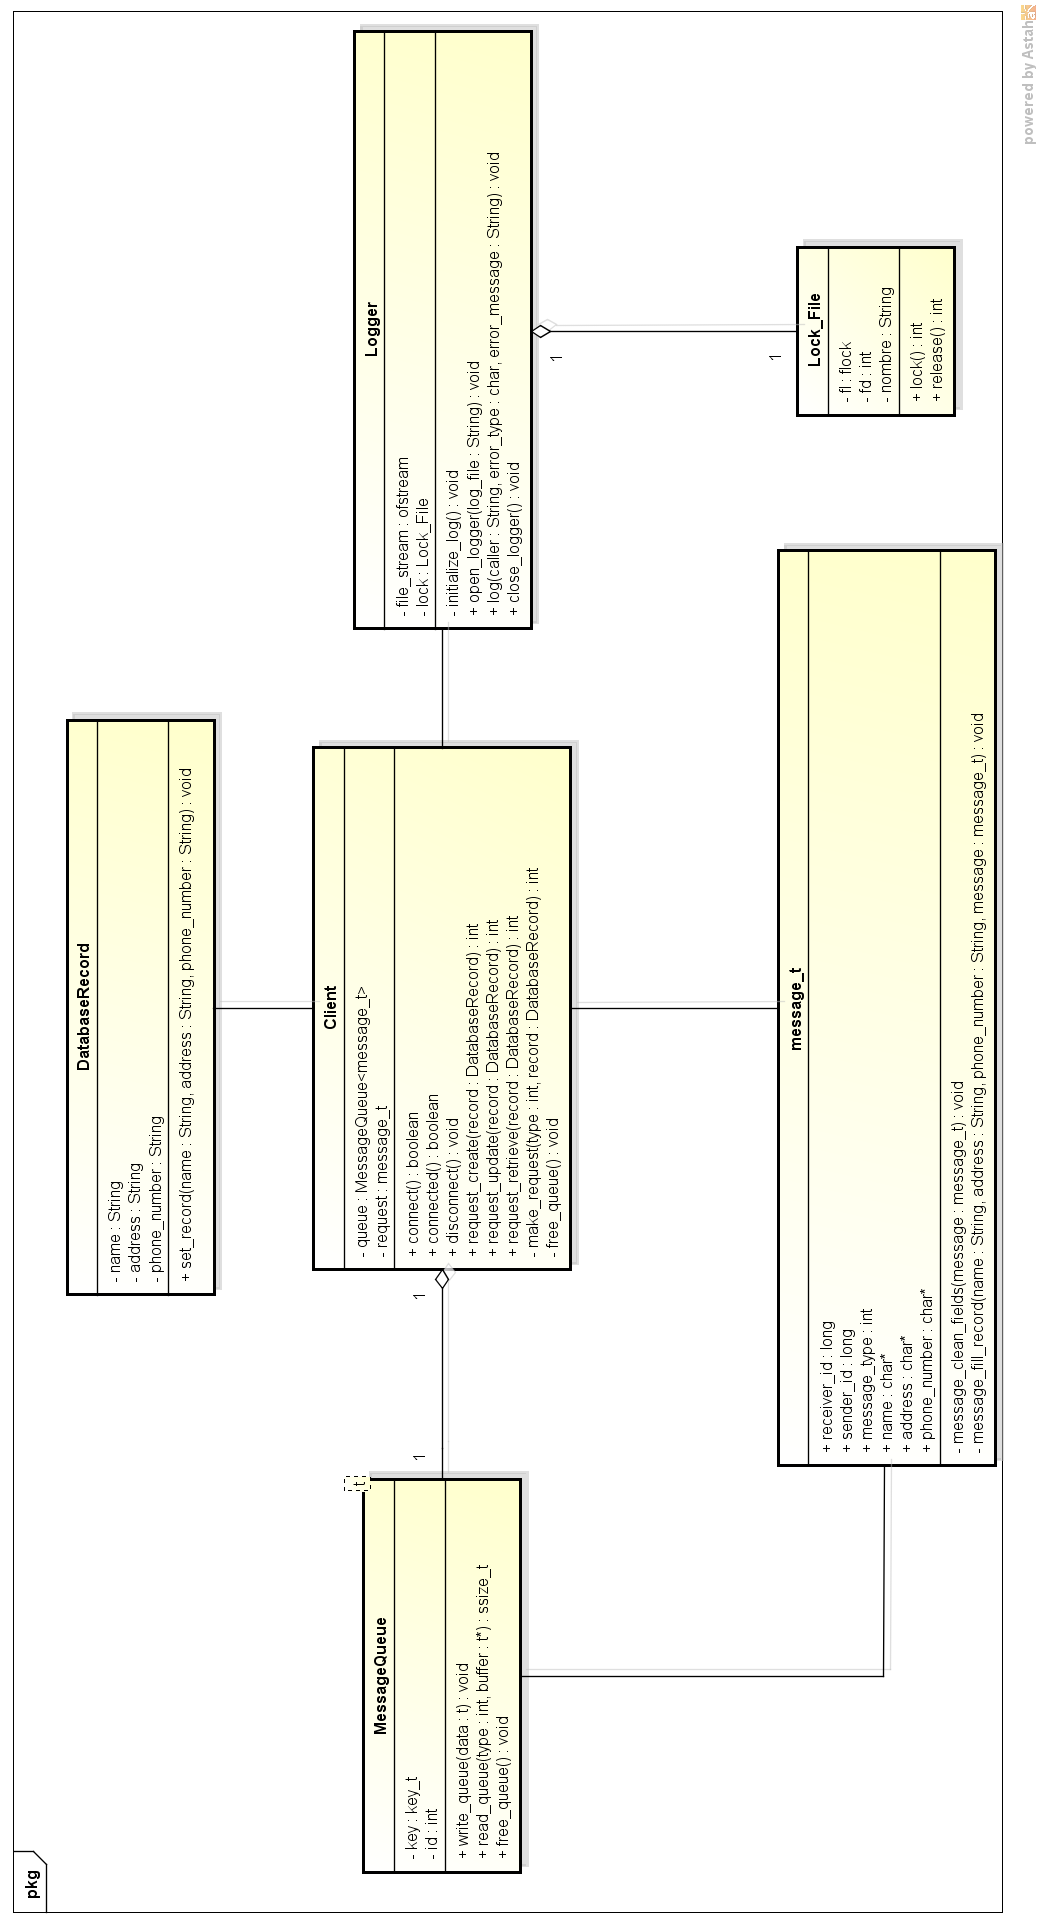
\includegraphics[width=360pt]{clases_cliente.png}
\caption{Diagrama de clases del cliente}
\end{center}
\end{figure}

\newpage

\begin{figure}[H]
\begin{center}
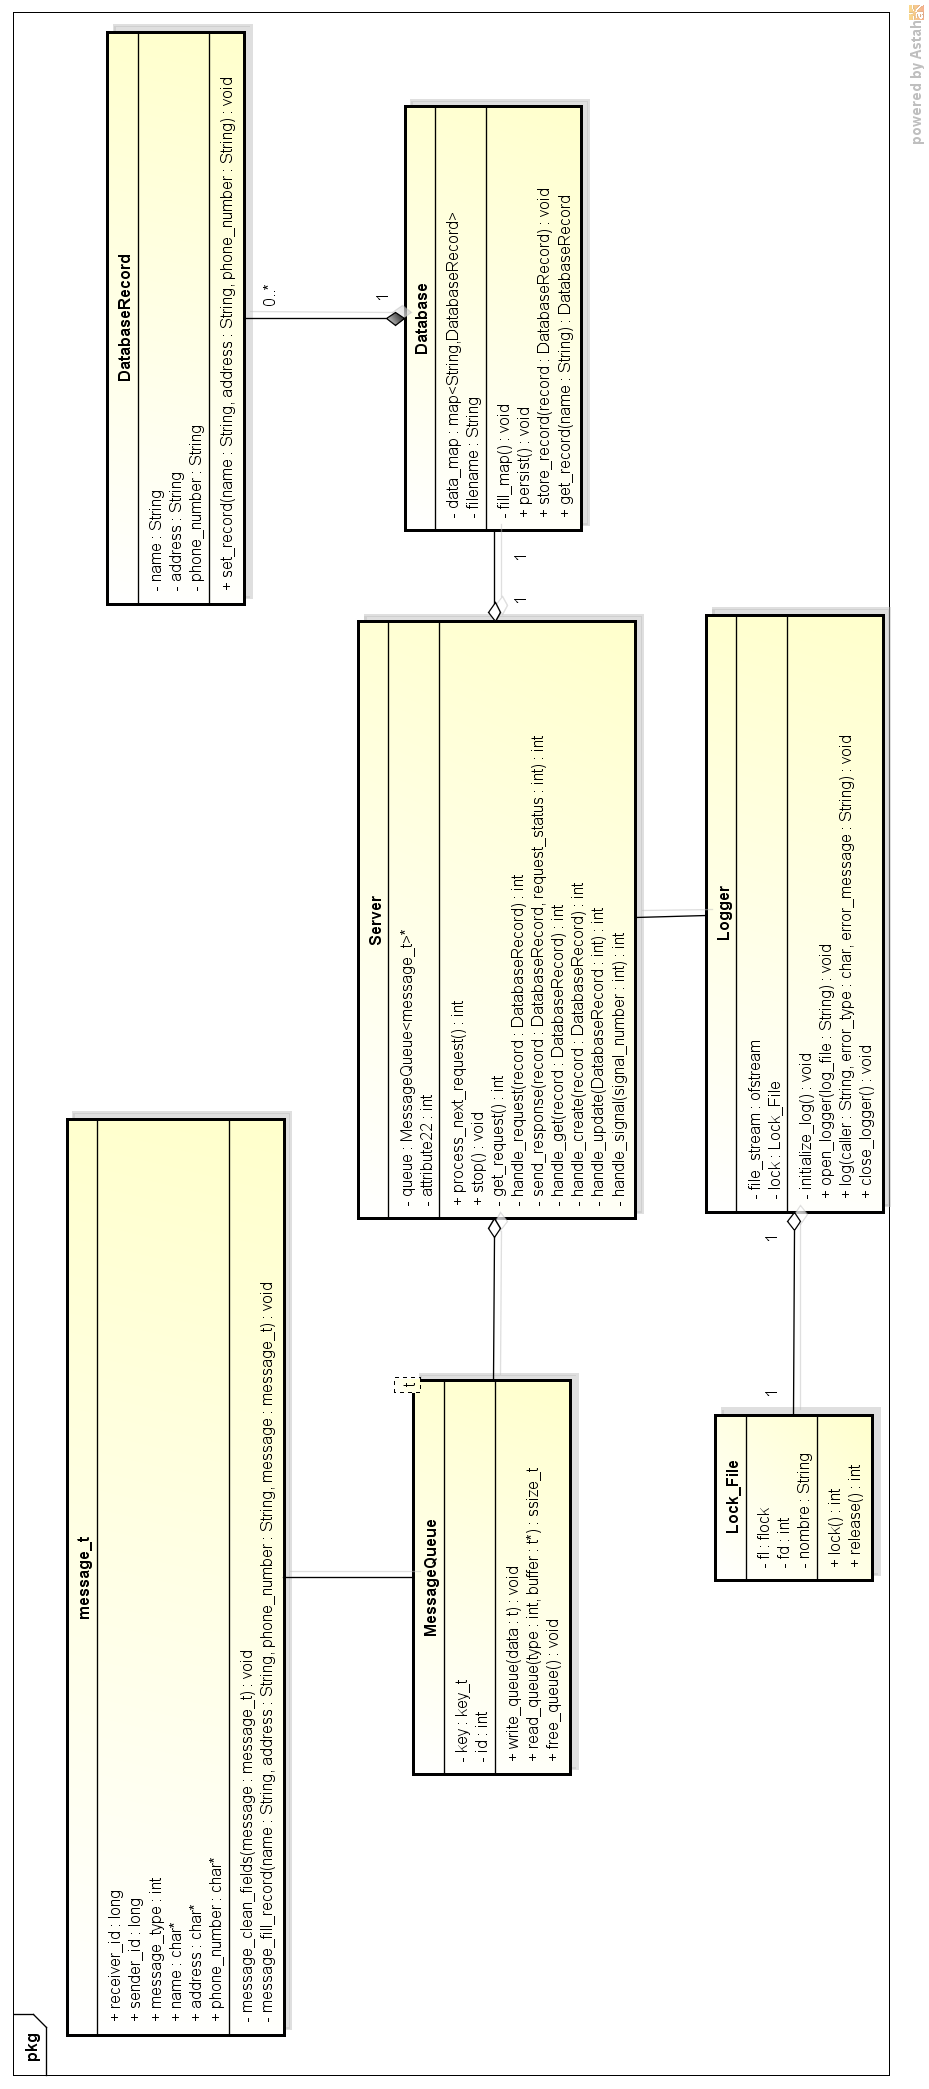
\includegraphics[width=310pt]{clases_servidor.png}
\caption{Diagrama de clases del servidor}
\end{center}
\end{figure}

\newpage

\section{Diagrama de casos de uso}

\begin{figure}[H]
\begin{center}
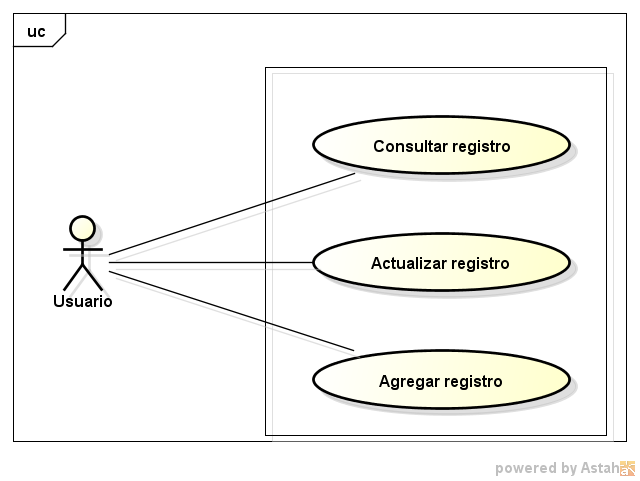
\includegraphics[width=350pt]{casos_uso.png}
\caption{Diagrama de casos de uso}
\end{center}
\end{figure}

\end{document}
